%\documentclass[11pt,hyperref={bookmarks=false}]{beamer}
%\documentclass[11pt,handout]{beamer}
\documentclass[11pt]{beamer}
%\usetheme{Copenhagen}
%\usetheme{default}
\usetheme{default}
%\usecolortheme{seagull}
\usefonttheme{professionalfonts}
%\useoutertheme{infolines}%{miniframes}
%\usepackage{xmpmulti}
%\usepackage{latexsym,fancyhdr,array,tabularx,multicol}
%\usepackage{ifthen,booktabs,calc,longtable,lscape,amsmath}
%\usepackage{egameps}
% \usepackage[usenames,dvipsnames]{pstricks}
% \usepackage{epsfig}
% \usepackage{pst-grad} % For gradients
% \usepackage{pst-plot} % For axes
%\usepackage{psfrag,graphicx}
\usepackage{graphicx,xfrac}
%\usepackage{xmpmulti}
\usepackage{latexsym,fancyhdr,array,tabularx,multicol,multirow}
\usepackage{booktabs}
\usepackage{amsmath}
\usepackage{subcaption}
\usepackage{changepage}
%\usepackage{multicol,ifthen,calc}
%\usepackage{multirow}
%\usepackage{pgf}
%\usepackage{longtable, lscape}
%\usepackage{lscape}
\newtheorem{df}{Definition}
\newtheorem{lm}{Lemma}
\newtheorem{prp}{Proposition}
\newtheorem{sprf}{Sketch of Proof}
\newtheorem{prf}{Proof}
\newtheorem{conjecture}{Conjecture}
\newtheorem{suffc}{Sufficient Condition}
\setbeameroption{hide notes}
\definecolor{tblue}{rgb}{0.2,0.2,0.7}

\AtBeginSection[]{%
  \frame<beamer>{ 
    \frametitle{Outline}   
    \tableofcontents[currentsection,currentsubsection] 
  }
}
%\newcommand{\threelinebracer}{$\left. \begin{array}{c} \\ \\ \\ \end{array} \right\rbrace$}
%\newcommand{\threelinebracel}{$\left. \begin{array}{c} \\ \\ \\ \end{array} \right\lbrace$}
%\newcommand{\twolinebracer}{$\left. \begin{array}{c} \\ \\ \end{array} \right\rbrace$}
%\newcommand{\twolinebracel}{$\left. \begin{array}{c} \\ \\ \end{array} \right\lbrace$}
\linespread{1.1}
%\setlength{\parindent}{0pt}
\usepackage{parskip}
\addtolength{\parskip}{0pt}
%\newenvironment{num}
% {\leftmargini=6mm\leftmarginii=8mm
	%  \begin{itemize}}{\end{itemize}}
% Separate slides by \begin{frame} and \end{frame}.
\title{The Allocation of Teaching Talent and \\Human Capital Accumulation}
\author[shortname]{Simeon Alder\inst{1} \and Yulia Dudareva\inst{2} \and Ananth Seshadri\inst{1}}
\institute[shortinst]{\inst{1} University of Wisconsin--Madison \and \inst{2} University of Stavanger Business School}

\date{\today}
\begin{document}
	
	\begin{frame}
		\titlepage
	\end{frame}
	
	\begin{frame}
		\frametitle{Introduction}
		\vfill
		\begin{itemize}
			\item Public education in U.S. has gone through major (positive) changes since end of WW II:
			\begin{itemize}
				\item[$\circ$] Annual real expenditures per student: \\
				\$2,100 (1950s) to \$12,000 (2010s)
				\item[$\circ$] Student-teacher ratio: 27 (1955) to 16 (2010s)
			\end{itemize}
			\vfill
			\item Evolution of educational outcomes doesn't compare favorably
with countries at similar income level (e.g. PISA assessments)
   %Evolution of educational outcomes doesn't compare favorably with countries at similar income level (e.g.~{\it PISA} assessments)
			\vfill
			\item Potential explanations include:
			\begin{itemize}
				\item[$\circ$] U.S.~education underfunded %by international comparison
				\item[$\circ$] Role of (powerful) teachers' unions \pause
				\item[$\circ$] \alert{Occupational choice} \pause
				\item[$\circ$] Local funding for public education (e.g.~property taxes)
			\end{itemize}
		\end{itemize}
		\vfill
	\end{frame}
	
	\begin{frame}
		\frametitle{Research Questions}
		\vfill
		\begin{itemize}
			\item To what extent do changes in career opportunities in other occupations affect selection of workers into teaching careers?
			\vfill
			\item To what extent are static efficiency gains associated with improved career opportunities in non-teaching occupations muted or amplified by dynamic effects?\\
			$\Rightarrow$ human capital accumulation channel
		\end{itemize}
		\vfill
	\end{frame}
	
	\begin{frame}
		\frametitle{What We Do}
		\vfill
		\begin{itemize}
			\item Highlight stylized facts
			\vfill
			\item Develop a novel theory of occupational choice and human capital formation: 
			\begin{itemize}
				\item[$\circ$] non-linear wages %$\Rightarrow$ comparative and absolute advantage
				\item[$\circ$] intergenerational dynamics of human capital accumulation
			\end{itemize}
			\vfill
			\item Combine three longitudinal surveys: 
			\begin{itemize}
				\item[$\circ$] Project TALENT, NLSY79, NLSY97
			    %\item[$\circ$] Occupation-specific abilities
            \end{itemize}
		\end{itemize}
		\vfill
	\end{frame}

%  \begin{frame}{Outline}
% \tableofcontents{}
% \end{frame}

%  \section{Stylized Facts}
	\begin{frame}
		\frametitle{Stylized Fact \#1}
		\framesubtitle{Majority of (Public) School Teachers is Female}
		\begin{table}[h!]
			\centering 
			\begin{tabular}{l l c }
				\toprule
				Time Period & & \% Female \\
				\midrule
				% after \\ : \hline or \cline{col1-col2} \cline{col3-col4} ...
                early 70s & Project TALENT  &  61.1 \\
                & Census 1980 &  59.8 \\
                1986-1993 & NLSY79  & 77.7   \\
                & Census 1990 & 74.8 \\
                2009-2013& NLSY97  & 77.1   \\
                & ACS 2009-2013  & 76.4  \\
				\midrule
				2003-2004 & NCES (2006) & 75\\
				\bottomrule
			\end{tabular}
		\end{table}
	\end{frame}
	
	\begin{frame}
		\frametitle{Stylized Fact \#2}
		\framesubtitle{Educational Barriers / Labor Market Discrimination}
		\begin{itemize}
			\item Females face low barriers / discrimination in teaching
			\item Barriers / discrimination in non-teaching occupations falling over time
		\end{itemize}
	\end{frame}
	
	\begin{frame}
		\frametitle{Stylized Fact \#3}
		\framesubtitle{Trends in Occupational Choice}
		\begin{itemize}
			\item Share of women in labor force who choose teaching: \\9.5\% in 1970 to 9.0\% in 2010
			\item Share of men in labor force who choose teaching: \\2.9\% in 1970 to 2.5\% in 2010
			\item Sharp rise in female labor force participation rate: \\33.8\% in 1970 to 64.4\% in 2010
			\item Decline in male labor force participation rate: \\87.5\% in 1970 to 77.1\% in 2010
		\end{itemize}
	\end{frame}

 	%  \begin{frame}
	 % 	\frametitle{Stylized Fact \#4}
	 % 	\framesubtitle{Trends in Ability Distribution of Females by Occupation}
	 % 	%\begin{adjustwidth}{2em}{2em}
	 % 		%\vfill
	 % 		\begin{figure}[ht!]
	 % 			\begin{subfigure}[b]{0.32\textwidth}
	 % 				\centering
	 % 				\includegraphics[width=\textwidth]{talent_afqt_female_no_lf.pdf}
	 % 			\end{subfigure}
	 % 			\begin{subfigure}[b]{0.32\textwidth}
	 % 				\centering
	 % 				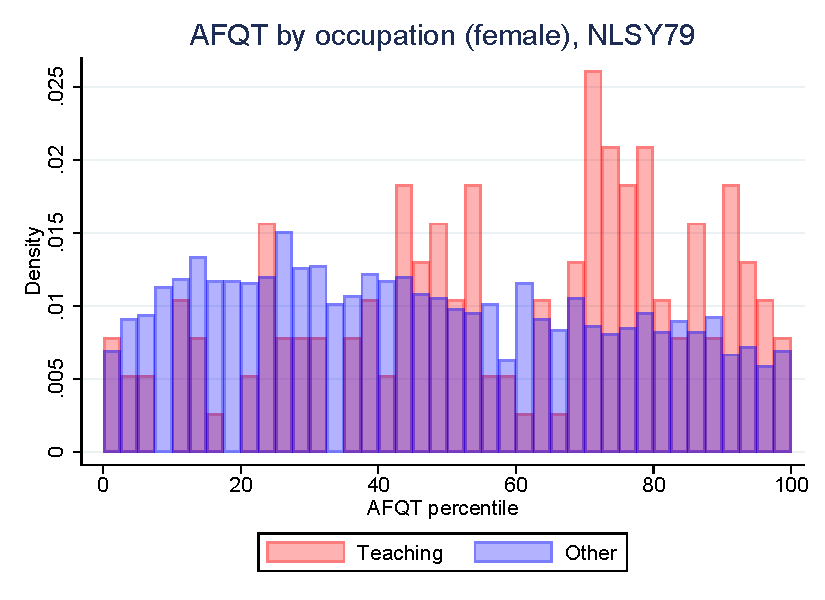
\includegraphics[width=\textwidth]{nlsy79_afqt_female_no_lf.pdf}
	 % 			\end{subfigure}
	 % 			\begin{subfigure}[b]{0.32\textwidth}
	 % 				\centering
	 % 				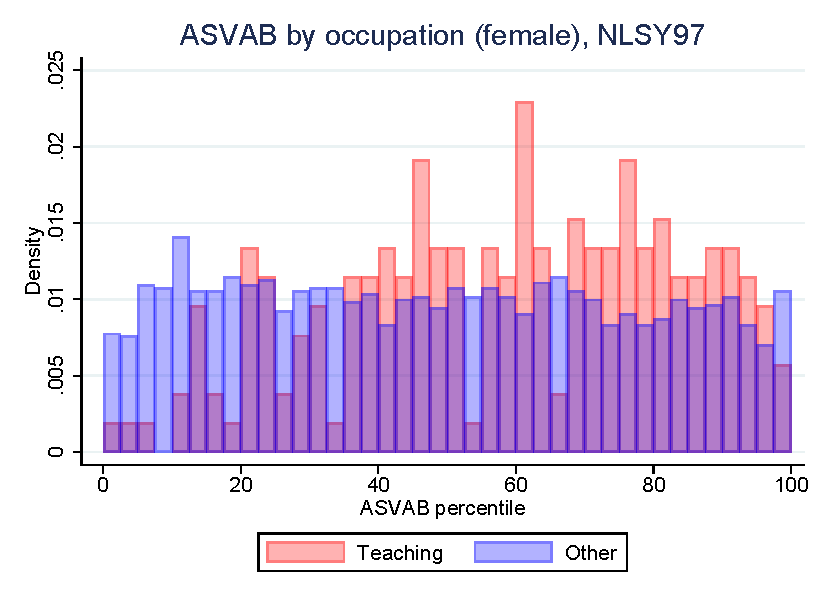
\includegraphics[width=\textwidth]{nlsy97_afqt_female_no_lf.pdf}
	 % 			\end{subfigure}		 			
	 % 		\end{figure}
	 % 		%\vfill
	 % 	%\end{adjustwidth}
	 % \end{frame}

	% \begin{frame}
	% 	\frametitle{Stylized Fact \#4}
	% 	\framesubtitle{Trends in Ability Distribution of Females by Occupation}
	% 	\begin{adjustwidth}{2em}{2em}
	% 		\vfill
	% 		\begin{figure}[ht!]
	% 			\begin{subfigure}[b]{0.27\textwidth}
	% 				\centering
	% 				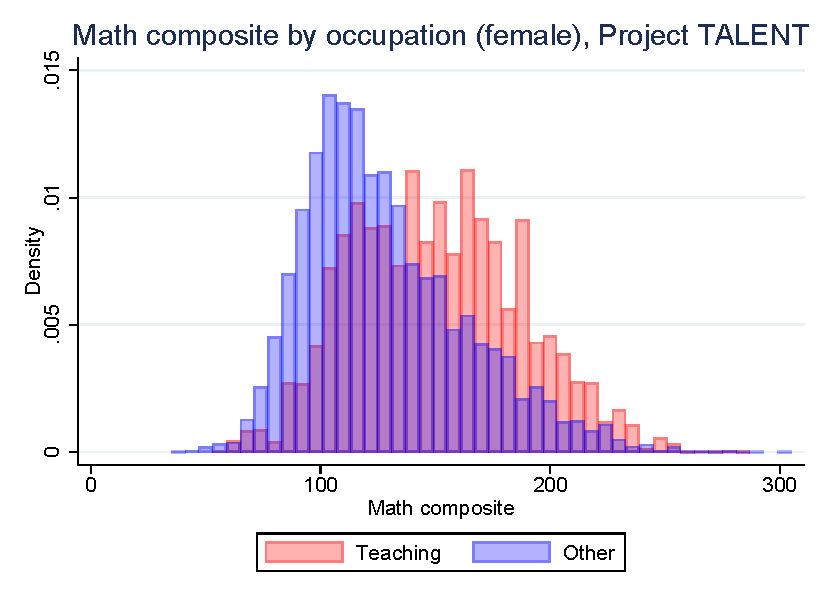
\includegraphics[width=\textwidth]{TALENT_math_occ_no_norm_female_no_lf.pdf}
	% 			\end{subfigure}
	% 			\hfill
	% 			\begin{subfigure}[b]{0.27\textwidth}
	% 				\centering
	% 				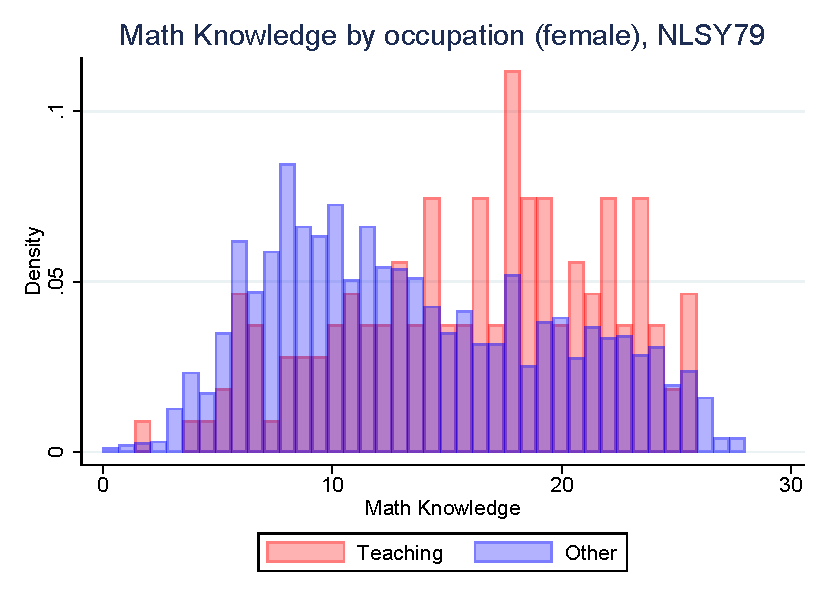
\includegraphics[width=\textwidth]{nlsy79_mk_occ_no_norm_female_no_lf.pdf}
	% 			\end{subfigure}
	% 			\hfill
	% 			\begin{subfigure}[b]{0.27\textwidth}
	% 				\centering
	% 				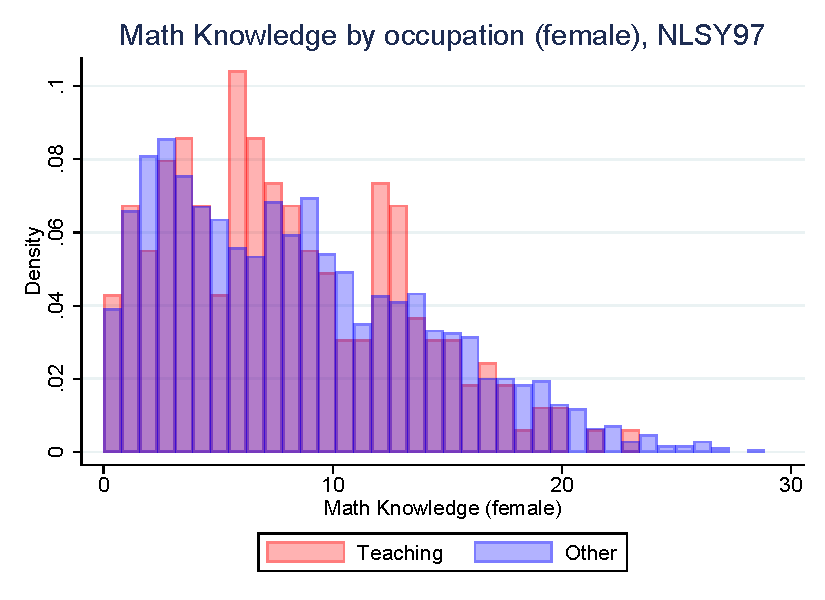
\includegraphics[width=\textwidth]{nlsy97_mk_occ_no_norm_female_no_lf.pdf}
	% 			\end{subfigure}	
	% 			\vfill	
	% 			\begin{subfigure}[b]{0.27\textwidth}
	% 				\centering
	% 				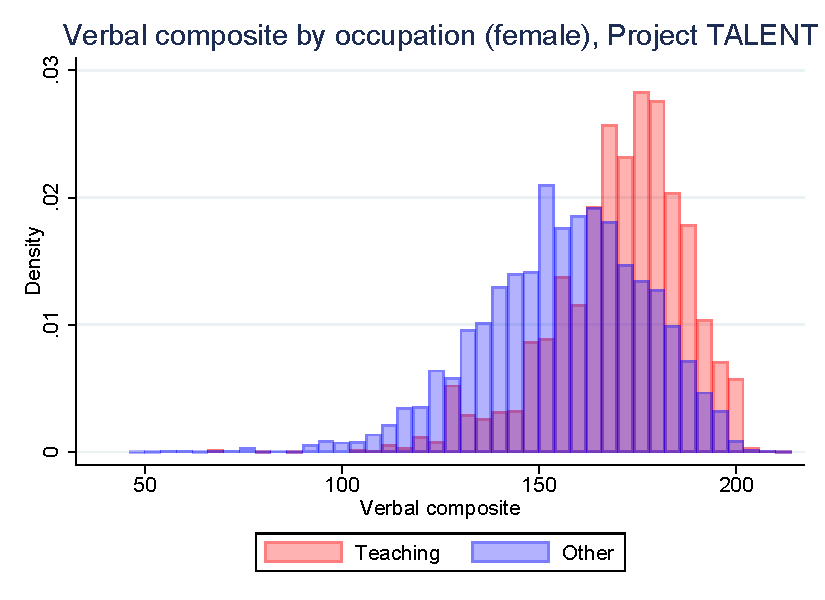
\includegraphics[width=\textwidth]{TALENT_verbal_occ_no_norm_female_no_lf.pdf}
	% 			\end{subfigure}
	% 			\hfill
	% 			\begin{subfigure}[b]{0.27\textwidth}
	% 				\centering
	% 				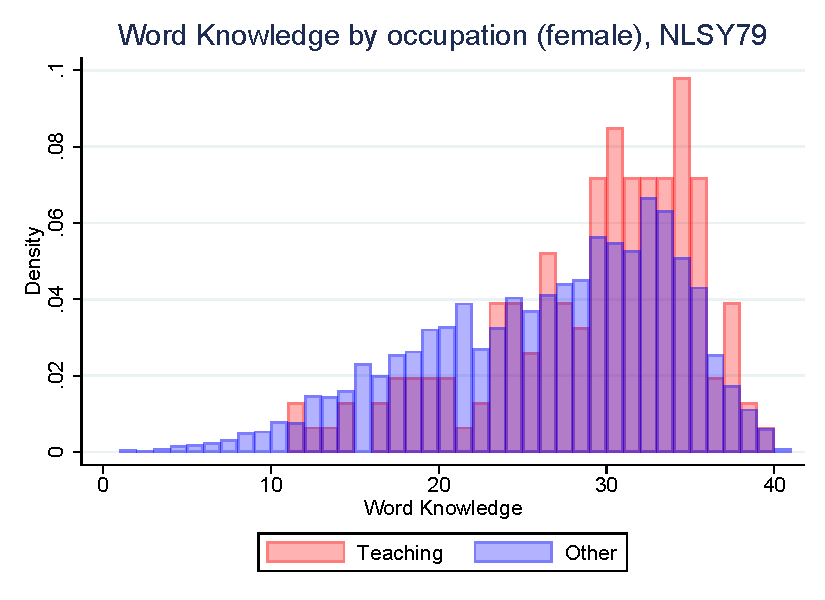
\includegraphics[width=\textwidth]{nlsy79_wk_occ_no_norm_female_no_lf.pdf}
	% 			\end{subfigure}
	% 			\hfill
	% 			\begin{subfigure}[b]{0.27\textwidth}
	% 				\centering
	% 				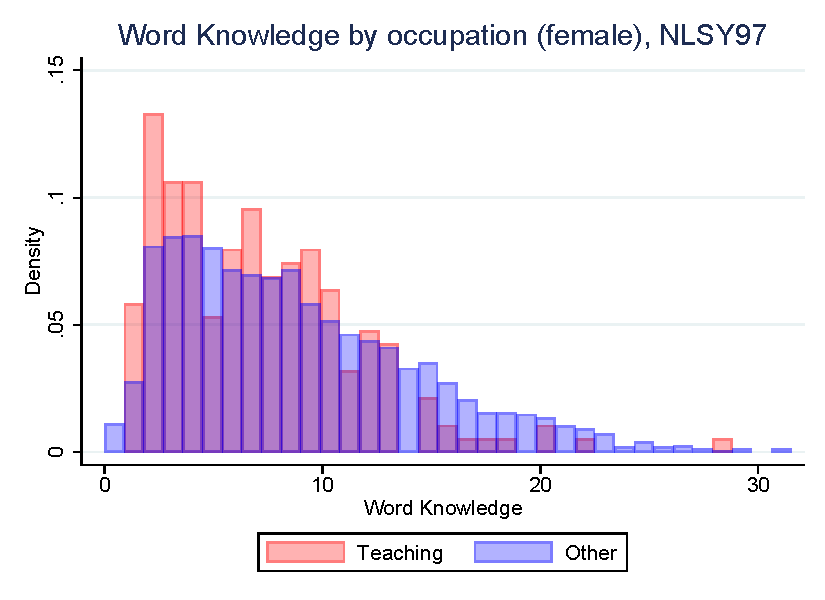
\includegraphics[width=\textwidth]{nlsy97_wk_occ_no_norm_female_no_lf.pdf}
	% 			\end{subfigure}	
	% 		\end{figure}
	% 		\vfill
	% 	\end{adjustwidth}
	% \end{frame}
	
%\section{Model}	
 \begin{frame}
		\frametitle{Model}
		\framesubtitle{Three Major Building Blocks}
		\begin{itemize}
			\item OLG with human capital investment
			\item Non-linear version of occupational choice model
			\item Educational barriers / labor market discrimination \\
			(as in Hsieh et al., 2019)
		\end{itemize}
	\end{frame}
	
	\begin{frame}
		\frametitle{Simple Two-Sector Model}
		\framesubtitle{Endowments, Preferences}
		\begin{itemize}
			\item Each period, a measure $M$ of agents is born and lives for two periods: ``young'' and ``old''
			\item $G=2$ groups of individuals
            \item $I=2$ occupations indexed by $i \in \{1,\dots,I\}$
			\item Occupational abilities $\vec{a}$ drawn from joint distribution $F(\vec{a})$
			\item $\log$ preferences over consumption and leisure:
			\begin{displaymath}
				\mu \ln C'_{g} + \ln\left(1-s_{i,g} \right)
			\end{displaymath}
		\end{itemize}
	\end{frame}
	
	\begin{frame}
		\frametitle{Simple Two-Sector Model}
		\framesubtitle{Technologies}
		\begin{itemize}
			\item ``Young'' make occupation-specific time and goods investments
			\item ``Old'' work as \alert{teachers} or \alert{production workers}
			%  \item Technologies are occupation-specific:
			\begin{description}
				\item[Human capital production] (teaching) depends on\\
				teacher's $h_{T,\hat{g}}$, class size $N(h_{T,\hat{g}})$,  own ability $a_i$, time $s_{i,g}$ and goods $e_{i,g}$ investments:
				\begin{align*}
					\label{}
					h'_{i,g}(a_i) & =\left( h_{T,\hat{g}}\right)^\beta a_i^\alpha(s_{i,g})^{\phi} (e_{i,g})^{\eta}\big(N(h_{T,\hat{g}})\big)^{-\sigma}
				\end{align*}
				\item[Final output production] depends on adult worker's human capital $h_{O,g}$ and exogenous productivity $A_O$:
				\begin{align*}
					\label{}
					y_g = A_O h_{O,g}
				\end{align*}
			\end{description}
		\end{itemize}
	\end{frame}

 \begin{frame}
		\frametitle{Simple Two-Sector Model}
        \framesubtitle{Education Sector}
		%\small
		%\begin{description}
		%  \item[Problem \#1:] We don't know $\omega(\cdot,\cdot)$ and we need to compute it numerically!
		%  \item[Challenge:] $\omega(\cdot,\cdot)$ is possibly non-linear in $h^T$ (for given $H^T$) 
		%  \item[Problem \#2:] For given $\omega(\cdot,\cdot)$, need to identify the fixed point $H^{T'} = {\widetilde{H^{T'}}} $.
		%  \item[Solution:] $\omega(\cdot,\cdot)$ is proportional to the \textit{number of students} in a teacher's class:
		%  \begin{equation*}
			%\omega(h^T,H^T) = \lambda N(h^T,H^T) = \lambda \frac{M}{2 H^T} \left( h^T \right)^{\frac{\beta}{\sigma}}
			%\end{equation*}
			\begin{itemize}
				\item Assignment of students to teachers is random \\ $\Rightarrow$ distribution of students' skill identical across classrooms
				\item Teachers with different $h_{T,g}$ vary with respect to class {\it size}
				\begin{align*}
                    N(h_{T,g})&=h_{T,g}^\frac{\beta}{\sigma} \cdot \frac{M}{2\widetilde{H}_T}\\
                    &\textrm{{\sf where }} \widetilde{H}_T =\sum_{\hat{g}=1}^G \int_0^\infty \left( h_{T,\hat{g}}\left( a \right) \right)^{\frac{\beta}{\sigma}} f_{T,\hat{g}}(a) da
				\end{align*}
				\item Teacher's wage $\omega_{T,g}$ depends on teacher's human capital:
				%\item $\omega(\cdot,\cdot)$ is proportional to the \textit{number of students} in a teacher's class:
				\begin{align*}
					\omega_T(h_{T,g})  =  \kappa h_{T,g}^\gamma 
					%\omega(h_{T,g},\widetilde{H}_T) & =  \lambda N(h^T,\widetilde{H}^T) \\
					%& = \frac{{H'}^O {A'}^O}{\frac{M}{2}\sum_{g=1}^G \int_0^\infty f_{O,g}(a) da} \cdot %\underbrace{\overbrace{N(1,\widetilde{H}^T)}^{=\frac{M}{2}\frac{1}{\widetilde{H}^T}}\left( h^T \right)^{\frac{\beta}{\sigma}}}_{=N(h^T,\widetilde{H}^T)} \\
					%& =\frac{\overbrace{{H}'_O {A}'_O}^{\textrm{total output (next period)}}}{\underbrace{\sum_{g=1}^G \int_0^\infty f_{O,g}(a) da}_{\begin{subarray}{c}\textrm{fraction of prospective} \\ 
					%\textrm{production workers in class}\end{subarray}}} \cdot \underbrace{\frac{\left( h_{T,g} \right)^{\frac{\beta}{\sigma}}}{{\widetilde{H}_T}}}_{\textrm{fraction of students taught}}\\ 
	\end{align*}
	%  \item $\lambda$ is the value of human capital per worker (in units of output) in occupation $O$.
\end{itemize}

%  \item[Implication:] standard Roy model results no longer hold
%\end{description}
\end{frame}
	
	
	\begin{frame}
		\frametitle{Simple Two-Sector Model}
		\framesubtitle{Values}
        \label{valuefn}
		\begin{align*}
			\label{}
			V_g(a_T,a_O,\widetilde{H}_T) & = \max_{\{s_{O,g},s_{T,g},e_{O,g},e_{T,g}\}} \bigg\{ V_{O,g}(a_O,\widetilde{H}_T), V_{T,g}(a_T,\widetilde{H}_T) \bigg\} \label{eq:V}
		\end{align*}
		where
		\begin{align*}
			%\label{eq:vo}
			V_{O,g}(a_O,\widetilde{H}_T) & = \ln\left(1-s_{O,g}\left(a_O,\widetilde{H}_T\right)\right) \nonumber \\
			& + \mu \ln \Big[ {{h'}_{O,g}} A_O'(1-t')\alert{(1-\tau^{\omega '}_{O,g})} \nonumber \\
			& - e_{O,g}(a_O,\widetilde{H}_T)(1+\tau^e_{O,g}) \Big],\\
			%\label{eq:vt}
			V_{T,g}(a_T,\widetilde{H}_T) & = \ln\left(1-s_{T,g}\left(a_T,\widetilde{H}_T\right)\right) \nonumber \\
			& + \mu \ln \Big[ \omega_{T,g}'({h_{T,g}'})(1-t')\alert{(1-\tau^{\omega '}_{T,g}) }\nonumber \\
			& - e_{T,g}(a_T,\widetilde{H}_T)(1+\tau^{e }_{T,g}) \Big] 
		\end{align*}
    \hyperlink{thresh}{\beamergotobutton{Occupational Threshold}}  \hyperlink{lom}{\beamergotobutton{Laws of Motion}}
	\end{frame}	

\begin{frame}
\frametitle{Equilibrium}
\label{eqm}
%\small
Given occupational choices of today's ``old'' and aggregate human capital $\widetilde{H}_{T}$ and ${H}_{O}$, the equilibrium consists of individual choices of ``young'' $\{e_{T,g}, s_{T,g}, e_{O,g}, s_{O,g}\}$, the occupational choice boundary $a^*_{T,g}(a_O)$, the corresponding densities $f_{T,g}$ and $f_{O,g}$, and occupation- and group-specific wage profiles $\{\omega_{T,g}, \omega_{O,g}\}$ such that:
\begin{enumerate}
	\item Individuals solve their investment and occupational choice problems \hyperlink{time_inv}{\beamergotobutton{Time Investment}} \hyperlink{good_inv}{\beamergotobutton{Goods Investment}}
	\item Aggregate human capital follows the laws of motion \hyperlink{laws}{\beamergotobutton{Laws of Motion}}
	\item Government budget constraint is satisfied \hyperlink{tax}{\beamergotobutton{Constraint}} 
\end{enumerate}
\end{frame}

\begin{frame}
\frametitle{Occupational Choice Boundary\ldots}
\framesubtitle{\ldots depends on aggregate state $\widetilde{H^T}$} 
%\footnotesize
\begin{align*}
	\frac{\alert{\bar{a}_T(a_O)}^\frac{\alpha}{\frac{1}{\gamma}-\eta}}{a_O^\frac{\alpha}{1-\eta}} \cdot \frac{s_{T,g}^\frac{\phi}{\frac{1}{\gamma}-\eta}}{s_{O,g}^\frac{\phi}{1-\eta}}\cdot \frac{\tau_{T,g}^\frac{1}{1-\eta\gamma}}{\tau_{O,g}^\frac{1}{1-\eta}} \cdot \frac{1+\tau^e_{T,g}}{1+\tau^e_{O,g}}\cdot \left(\frac{1-s_{T,g}}{1-s_{O,g}}\right)^\frac{1}{\mu} \nonumber\\
	\times \frac{\left(\kappa \cdot \gamma\right)^\frac{1}{1-\eta\gamma}}{{A'}_O^\frac{1}{1-\eta}} \cdot \frac{\frac{1}{\gamma}-\eta}{1-\eta}\cdot \eta^\frac{\eta(\gamma-1)}{(1-\eta)(1-\eta\gamma)} \cdot \left(\tfrac{2\alert{\widetilde{H}_T}}{M}\right)^{\frac{\sigma(\alert{\gamma}-1)}{(1-\eta)(1-\eta\gamma)}}=1 \nonumber
\end{align*}
where
\begin{align}
	\tau_{i,g} =\frac{(1-t)(1-\tau^{\omega}_{i,g})}{1+\tau^e_{i,g}} \nonumber
\end{align}
\end{frame}

%\section{Data}	
\begin{frame}
\frametitle{Data}
%\framesubtitle{}
\begin{itemize}
	\item Micro-data on abilities and occupational choice:
	\begin{enumerate}
		\item Project TALENT (1960-1975):
		\begin{itemize}
			\item representative 5\% sample of high school population in 1960
			\item follow-up surveys at 1, 5, and 11-year post graduation
		\end{itemize}
		\item NLSY 79
		\item NLSY 97
	\end{enumerate}
	\item \textit{Math}, \textit{Verbal}, and \textit{Social} abilities
	\item Occupational choice 11 years after (likely) high school graduation in all surveys ($\sim$ age 29)
\end{itemize}
\end{frame}

%\section{Calibration}	
\begin{frame}
\frametitle{Calibration}
\label{calib}
Calibrate to 1970, 1990, and 2010: 2 groups, 21 sectors
\begin{itemize}
\item Assumptions: no barriers for men, no barriers for women in teaching \hyperlink{assump}{\beamergotobutton{Assumptions}}
\item Time-invariant parameters: match wage dispersion, educational attainment and investment \hyperlink{invar}{\beamergotobutton{Time-Invariant}}
\item Time-varying parameters: match occupational shares \hyperlink{var}{\beamergotobutton{Time-Varying}}
\end{itemize}
\end{frame}

\begin{frame}
\frametitle{Preliminary Results}
\label{res}
\begin{itemize}
    \item Ability composition of teachers change over time:
    \begin{itemize}
				\item[$\circ$] Women with lower ability become teachers \hyperlink{femaleabil}{\beamergotobutton{Distribution of Abilities (female)}} % because other careers are more attractive
                \item[$\circ$] Men with higher ability become teachers\\ \hyperlink{maleabil}{\beamergotobutton{Distribution of Abilities (male)}} % because other careers are more attractive
    \end{itemize}
    \item Human capital investment decline over time, given ability \hyperlink{invest}{\beamergotobutton{HC Investment}} % because lower ability and lower wages
    %\item $\Rightarrow$ Lower average teaching human capital 
    \item More women become teachers
    \item Fewer men become teachers
    %\item Smaller class sizes
    \item $\Rightarrow$ Same level of aggregate teaching human capital \hyperlink{humcap}{\beamergotobutton{HC}}
    %\item $\Rightarrow$ Lower non-teaching output
\end{itemize}
\end{frame}

%\section{Counterfactual}
\begin{frame}
\frametitle{Counterfactual Experiment 1}
\begin{itemize}
  \item "Freeze" women's occupational barriers at 1970 level (i.e., $\tau_w$ constant over time)
  \item Use occupational productivities from benchmark calibration
  %\item Adjust value of $\kappa$ to match men's occupational choices from benchmark calibration.
\end{itemize}
\end{frame}

\begin{frame}
\frametitle{Counterfactual 1: Results}
\label{count}
\begin{itemize}
    \item Ability composition of teachers differ:
    \begin{itemize}
				\item[$\circ$] Women with (relatively) higher ability become teachers \hyperlink{counter_femaleabil}{\beamergotobutton{Distribution of Abilities (female)}} % because other careers are more attractive
                \item[$\circ$] Men with (relatively) lower ability become teachers
                \hyperlink{counter_maleabil}{\beamergotobutton{Distribution of Abilities (male)}}% because other careers are more attractive
    \end{itemize}
    \item Human capital investment is (relatively) lower, given ability \hyperlink{counter_invest}{\beamergotobutton{HC Investment}} % because lower ability and lower wages
    %\item $\Rightarrow$ Lower average teaching human capital 
    \item (Relatively) fewer women become teachers
    \item (Relatively) more men become teachers
    %\item Smaller class sizes
    \item $\Rightarrow$ (Relatively) lower level of aggregate teaching human capital  \hyperlink{counter_humcap}{\beamergotobutton{HC}}
    %\item $\Rightarrow$ (Relatively) lower non-teaching output 
\end{itemize}
\end{frame}

% \begin{frame}
% \frametitle{Counterfactual Experiment 2}
% \begin{itemize}
%   \item Women face no barriers (i.e., $\tau_w=0$)
%   \item Use occupational productivities from benchmark calibration
%   %\item Adjust value of $\kappa$ to match men's occupational choices from benchmark calibration.
% \end{itemize}
% \end{frame}

% \begin{frame}
% \frametitle{Counterfactual 2: Results}
% \label{count2}
% \begin{itemize}
%     \item Ability composition of teachers differ:
%     \begin{itemize}
% 				\item[$\circ$] Women with (relatively) higher ability become teachers \hyperlink{counter2_femaleabil}{\beamergotobutton{Distribution of Abilities (female)}} % because other careers are more attractive
%                 \item[$\circ$] Men with same ability become teachers
%                 \hyperlink{counter2_maleabil}{\beamergotobutton{Distribution of Abilities (male)}}% because other careers are more attractive
%     \end{itemize}
%     \item Human capital investment is (relatively) lower, given ability \hyperlink{counter2_invest}{\beamergotobutton{HC Investment}} % because lower ability and lower wages
%     %\item $\Rightarrow$ Lower average teaching human capital 
%     \item (Relatively) fewer women become teachers
%     \item (Relatively) more men become teachers
%     %\item Smaller class sizes
%     \item $\Rightarrow$ (Relatively) lower level of aggregate teaching human capital  \hyperlink{counter2_humcap}{\beamergotobutton{HC}}
%     %\item $\Rightarrow$ (Relatively) lower non-teaching output 
% \end{itemize}
% \end{frame}

\begin{frame}
	\frametitle{Conclusion}
	%\framesubtitle{}
 \small
	\textcolor{tblue}{Results}
	\begin{itemize}
		\item Develop a novel theory of occupational choice and human capital formation: 
		\begin{itemize}
			\item[$\circ$] non-linear wages %$\Rightarrow$ comparative and absolute advantage
			\item[$\circ$] intergenerational dynamics of human capital accumulation
		\end{itemize}
        \item Combine Project TALENT, NLSY79, NLSY97
		%\item Calibrate change in barriers
	\end{itemize}
	\textcolor{tblue}{Ongoing and Future Work}
	\begin{itemize}	
        \item Decomposition:
            \begin{itemize}
			\item[$\circ$] static gains (as in Hsieh et al., 2019) vs.
			\item[$\circ$] dynamic effects (human capital accumulation)
		\end{itemize}
		\item Multiple locations differentiated by amenities and/or local tax rates (implicit school segregation by income)
	\end{itemize}
\end{frame}

\begin{frame}
	\frametitle{Occupations} 
	\label{occupations}
 \scriptsize
	\begin{enumerate}
\item Executives, Administrative, and Managerial
\vspace{-0.2cm}
\item Management Related
\vspace{-0.2cm}
\item Architects, Engineers, Math, and Computer Science
\vspace{-0.2cm}
\item Natural and Social Scientists, Recreation, Religious, Arts, Athletes
\vspace{-0.2cm}
\item Doctors and Lawyers
\vspace{-0.2cm}
\item Nurses, Therapists, and Other Health Service
\vspace{-0.2cm}
\item Teachers, Postsecondary
\vspace{-0.2cm}
\item Teachers, Non-Postsecondary and Librarians
\vspace{-0.2cm}
\item Health and Science Technicians
\vspace{-0.2cm}
\item Sales, All
\vspace{-0.2cm}
\item Administrative Support, Clerks, Record
\vspace{-0.2cm}
\item Fire, Police, and Guards
\vspace{-0.2cm}
\item Food, Cleaning, and Personal Services and Private Household
\vspace{-0.2cm}
\item Farm, Related Agriculture, Logging, and Extraction
\vspace{-0.2cm}
\item Mechanics and Construction
\vspace{-0.2cm}
\item Precision Manufacturing
\vspace{-0.2cm}
\item Manufacturing Operators
\vspace{-0.2cm}
\item Fabricators, Inspectors, and Material Handlers
\vspace{-0.2cm}
\item Vehicle Operators
\vspace{-0.2cm}
\item Home Production 
	\end{enumerate}
\end{frame}

\begin{frame}
\frametitle{Law of Motion}
\begin{figure}
\begin{center}
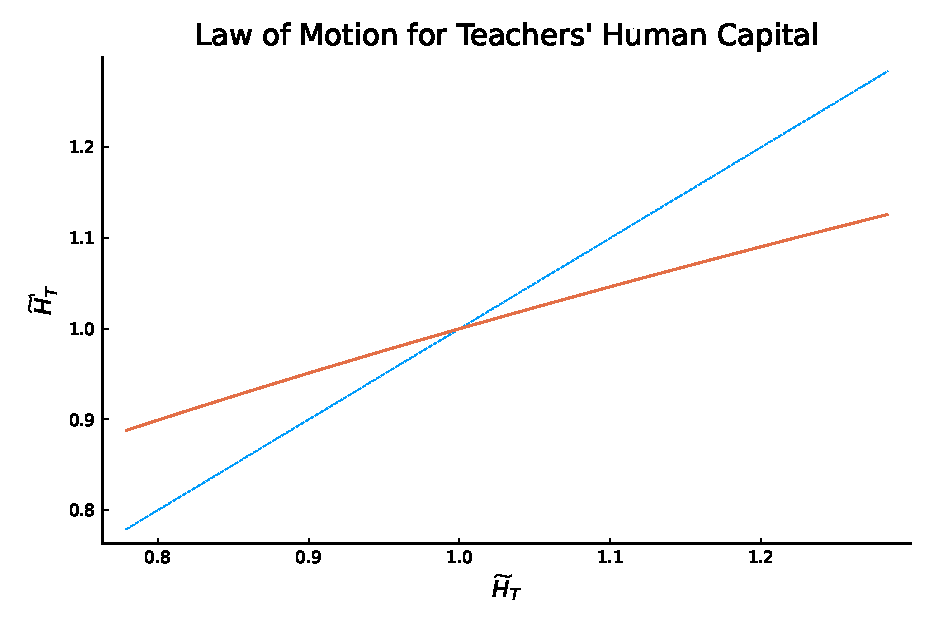
\includegraphics[width=0.8\textwidth]{LoM.eps}
%\caption{ }
\label{ }
\end{center}
\end{figure}
\end{frame}

\begin{frame}
		\frametitle{Simple Two-Sector Model}
		\framesubtitle{Occupational Threshold}
        \label{thresh}
		\begin{equation*}
			%\label{eq:ot}
			a^*_{T,g}(a_O) = \bar{a}_g\big(a_{O},\widetilde{H}_T\big) %\\
		\end{equation*}
		such that
		\begin{equation}
			\label{eq:indiff}
			V_{O,g}(a_{O},\widetilde{H}_T) = V_{T,g}\left(a^*_{T,g}(a_O),\widetilde{H}_T\right) \textrm{{\sf , for all} } a_O \in (0,\infty) \nonumber
		\end{equation}
  \hyperlink{valuefn}{\beamergotobutton{Back}}
	\end{frame}
	
	\begin{frame}
		\frametitle{Simple Two-Sector Model}
		\framesubtitle{Constraints}
        \label{tax}
		\begin{align*}
			%H^{T} & = \int_{0}^{\infty} \left(h^{T}(a)\right)^{\frac{\beta}{\sigma}} f^{T}(a) da \\
			\alert{t}\Bigg[ \sum_{g=1}^G \int_0^\infty (1-\tau^{\omega}_{T,g})\omega_{T,g}\left(h_{T,g}(a)\right) f_{T,g}(a) da  \\
			+ \sum_{g=1}^G \int_0^\infty (1-\tau^{\omega}_{O,g})A_O h_{O,g}(a) f_{O,g}(a) da \Bigg]\\
			= \sum_{g=1}^G \int_0^\infty (1-\tau^{\omega}_{T,g})\omega_{T,g}\left(h_{T,g}(a)\right) f_{T,g}(a) da \\
			f_{T,g}(a)  = \int_0^{\bar{a}_g^{-1}\left(a\right)} f\big(a,b \big) db \\
			f_{O,g}(b)  = \int_0^{\bar{a}_g\left(b\right)} f\big(a,b \big) da 
			%f^T(a) & = \int_0^{\bar{a}\big(a;H^T,{H^T}'\big)} f\big(a,a^O\big) da^O 
		\end{align*}	
  \hyperlink{eqm}{\beamergotobutton{Back}}
	\end{frame}

 \begin{frame}
		\frametitle{Simple Two-Sector Model}
		\framesubtitle{Laws of Motion}
  \label{lom}
		\begin{align*}
			{H}_{O}' & = \sum_{g=1}^G \int_0^\infty \left(\tfrac{2 \widetilde{H}_T}{M}\right)^\sigma a^\alpha s_{O,g}\left(a,\widetilde{H}_T\right)^\phi e_{O,g}(a,\widetilde{H}_T)^\eta  f_{O,g}(a) da \\
			\widetilde{H}_{T}' & = \sum_{g=1}^G \int_0^\infty \left(\left(\tfrac{2 \widetilde{H}_T}{M}\right)^\sigma a^\alpha s_{T,g}\left(a,\widetilde{H}_T\right)^\phi e_{T,g}(a,\widetilde{H}_T)^\eta \right)^{\alert{\frac{\beta}{\sigma}}} f_{T,g}(a) da 
		\end{align*}
  \hyperlink{valuefn}{\beamergotobutton{Back}}
	\end{frame}

\begin{frame}
	\frametitle{Optimal Time Investment} 
	\label{time_inv}
	%The F.O.C.s for $s^T$ and $e^T$, respectively, after a few steps of algebra are:
	\begin{align}
		%\label{eq:s_T}
		s_{T,g} & = \frac{\mu \phi}{\mu \phi+\tfrac{1}{\gamma}-\eta} \nonumber\\
		%\label{eq:e_T}
		s_{O,g} & = \frac{\mu \phi}{\mu \phi+1-\eta} \nonumber
	\end{align}
	\hyperlink{eqm}{\beamergotobutton{Back}}
\end{frame}

\begin{frame}
	\frametitle{Optimal Goods Investment} 
	\label{good_inv}
	%The F.O.C.s for $s^T$ and $e^T$, respectively, after a few steps of algebra are:
	\begin{align}
		%\label{eq:s_T}
		e_{T,g} & = \left( \left(\kappa \cdot \gamma \cdot \eta \cdot \tau_{T,g} \right)^\frac{1}{\gamma} \cdot a_T^{\alpha} \cdot s_{T,g}^{\phi} \cdot \left(\tfrac{2\widetilde{H}_T}{M}\right)^{\sigma}\right)^{\frac{1}{\frac{1}{\gamma}-\eta}}  \nonumber\\
		%\label{eq:e_T}
		e_{O,g} & = \left( {{A'}_{O}} \cdot \eta \cdot\tau_{O,g} \cdot a_O^\alpha \cdot s_{O,g}^\phi \cdot  \left(\tfrac{2\widetilde{H}_T}{M}\right)^\sigma \right)^{\frac{1}{1-\eta}} \nonumber
	\end{align}
	where
	\begin{align}
		\tau_{i,g} =\frac{(1-t)(1-\tau^{\omega}_{i,g})}{1+\tau^e_{i,g}} \nonumber
	\end{align}
	\hyperlink{eqm}{\beamergotobutton{Back}}
\end{frame}

\begin{frame}
	\frametitle{Aggregate Laws of Motion} 
	\label{laws}
	\small
	%The F.O.C.s for $s^T$ and $e^T$, respectively, after a few steps of algebra are:
	\begin{align}
		%\label{eq:lomT}
		\widetilde{H}'_{T} & = \Bigg[ \left(\kappa \cdot \gamma \cdot \eta\right)^{\frac{\eta}{1-\eta\gamma}} \cdot \left(\tfrac{2\widetilde{H}_T}{M}\right)^{\frac{\sigma}{1-\eta\gamma}}\nonumber\\
		& \times \sum_{g=1}^G \tau_{T,g}^\frac{\eta}{1-\eta\gamma} \cdot \int_0^\infty  s_{T,g}^\frac{\phi}{1-\eta\gamma} \cdot a^\frac{\alpha}{1-\eta\gamma}  f_{T,g}(a)da \Bigg]^\frac{\beta}{\sigma} \nonumber\\  
		%\Bigg[ \left(\tfrac{\beta}{\sigma}\right)^\eta \cdot\eta^{\frac{1}{1-\eta}} \cdot \left(\tfrac{2\widetilde{H}_T}{M}\right)^{\frac{\sigma}{1-\eta}} \nonumber\\
		%& \times \Bigg( \frac{\sum_{i=2}^I \sum_{g=1}^G {A_i'}^\frac{1}{1-\eta}\cdot\tau_{i,g}^\frac{\eta}{1-\eta} \cdot s_{i,g}^\frac{\phi}{1-\eta}\cdot \int_0^\infty a^{\frac{\alpha}{1-\eta}} f_{i,g}(a)da}{\sum_{i=2}^I \sum_{g=1}^G f_{i,g}(a)da} \Bigg)^\eta \nonumber\\
		%& \times \Bigg(\sum_{g=1}^G \tau_{T,g}^\frac{\eta\beta }{\sigma-\eta\beta } \cdot s_{T,g}^\frac{\phi\beta }{\sigma-\eta\beta } \cdot \int_0^\infty a^\frac{\alpha\beta}{\sigma-\eta\beta } f^{g,T}(a)da \Bigg)^\frac{\sigma-\eta\beta}{\beta} \Bigg]^\frac{\beta}{\sigma} \nonumber\\
		{H}'_{O} & = \left({A'}_O \cdot \eta\right)^\frac{\eta}{1-\eta} \cdot \left(\tfrac{2\widetilde{H}_T}{M}\right)^\frac{\sigma}{1-\eta} \cdot  \sum_{g=1}^G \tau_{O,g}^\frac{\eta}{1-\eta} \cdot \int_0^\infty s_{O,g}^\frac{\phi}{1-\eta} \cdot a^{\frac{\alpha}{1-\eta}} f_{O,g}(a)da \nonumber
		%\sum_{g=1}^G \left( \tau_{O,g}^\eta \cdot \eta^\eta \cdot \left(\tfrac{2\widetilde{H}_T}{M}\right)^\frac{\sigma}{1-\eta}\cdot {A'}_O^\eta \cdot s_{T,g}^\phi \right)^\frac{1}{1-\eta}\cdot \int_0^\infty a^{\frac{\alpha}{1-\eta}} f_{O,g}(a)da \nonumber
	\end{align}
	where
	\begin{align}
		\tau_{i,g} =\frac{(1-t)(1-\tau^{\omega}_{i,g})}{1+\tau^e_{i,g}} \nonumber
	\end{align}
	\hyperlink{eqm}{\beamergotobutton{Back}}
\end{frame}

\begin{frame}
\frametitle{Calibration}
\framesubtitle{Assumptions and Normalizations}
\label{assump}
  \tiny
%			\begin{itemize}
	%  \item $o \in \{1,\ldots,O\}$: index for non-teaching occupations 
	%  \item $T$: index for teaching
	%\end{itemize}
	
	\begin{table}[h!]
		\centering
		\begin{tabular}{lccc}
			\toprule
			Parameter & Definition & Determination & Value\\
			\midrule
			$\tau^{w}_{o,{\rm men}}$ & labor market barriers for men & assumption & 0 \\
			$\tau^{e}_{o,g}$ & human capital barriers for all groups & assumption & 0 \\
			$\tau^{w}_{T,g}$ & labor market barriers in teaching  & assumption & 0 \\
			& (all groups)&\\
			$\tau^{e}_{T,g}$ & human capital barriers in teaching & assumption & 0 \\
			& (all groups) & \\
			$\alpha$ & elasticity of human capital with respect to & normalization & 1 \\
			& idiosyncratic ability & \\
            $A_{12}$ & productivity in "Fire, Police,..." & normalization & 1 \\
   \midrule
   			$\beta$ & elasticity of human capital with respect to & free parameter & 0.5\\
    & teacher's human capital & \\
            $\sigma$ & elasticity of human capital with respect to & free parameter & 0.5 \\
            & class size & \\
			%					$\tau^{e}_{i,g}$ & Human capital barriers for other groups & Normalization & 0 \\
			%					$A_{T}$ & Teachers productivity & Normalization & 1 \\
			%					$\mu_a$ & Mean ability distribution & Normalization & 0 \\
			%					$\sigma_a$ & St.dev. ability distribution & Normalization & 1 \\
			\bottomrule
			%			\bottomrule
		\end{tabular}
		%\caption{Assumptions and Normalization}
		\label{tab:assump}
	\end{table}
  \hyperlink{calib}{\beamergotobutton{Back}}
\end{frame}

\begin{frame}
	\frametitle{Calibration}
	\framesubtitle{Time-Invariant Parameters}
 \label{invar}
	\tiny
	\begin{table}[h!]
		\centering
		\begin{tabular}{lccc}
			\toprule
			Parameter & Definition & Determination & Value\\
			\midrule
			$\theta$ & shape parameter of Fr\'echet-distributed & wage dispersion & 1.476\\
			& idiosyncratic abilities & in non-teaching occupations &\\
			%					\midrule
			$\eta$ & goods elasticity of human capital & aggregate education spending share  & 0.103\\
			%					\midrule
			$\phi$ & time elasticity of human capital & years of education  & 1.028\\
            &  & (non-teaching) &\\
			%					\midrule
			$\gamma$ & curvature of wage function in teaching & wage dispersion in teaching & 0.83\\
			%\midrule
			$\mu$ &  trade-off between consumption and & Mincerian returns to education & 0.714\\
			& time spent accumulating human capital & (non-teaching) & \\
			\bottomrule
			%			\bottomrule
		\end{tabular}
		%\caption{Baseline Parameter Values}
		\label{tab:param}
	\end{table}
 \hyperlink{calib}{\beamergotobutton{Back}}
\end{frame}

\begin{frame}
	\frametitle{Calibration}
	\framesubtitle{Time-Varying Parameters}
  \label{var}
	\tiny
	\begin{table}[h!]
		\centering
		\begin{tabular}{lcc}
			\toprule
			%					\toprule
			Parameter & Definition & Determination \\
			\midrule			
			$A_{o}$ & occupational productivities (non-teaching) & labor market shares for men  \\
			%					\midrule
			$\tau^{w}_{o,{\rm women}}$ & labor market barriers (non-teaching) & labor market shares for women \\
			& faced by women & \\
			%					\midrule
			$\kappa$ & scale parameter of wage function in teaching & fraction of males who are teachers \\
			%					\midrule
			$\lambda_f$ & aggregate labor market barrier for women & fraction of females who are teachers \\
			& in non-teaching occupations & \\
			% s_T/s_O, where  s_i=years of school/25 years
			\bottomrule
			%			\bottomrule
		\end{tabular}
		%\caption{Baseline Parameter Values}
		\label{tab:param_time}
	\end{table}
 \hyperlink{calib}{\beamergotobutton{Back}}
\end{frame}

\begin{frame}
\frametitle{Distribution of Teaching Abilities}
\framesubtitle{Female workers with lower abilities become teachers}
\label{femaleabil}
\begin{figure}
 \begin{center}
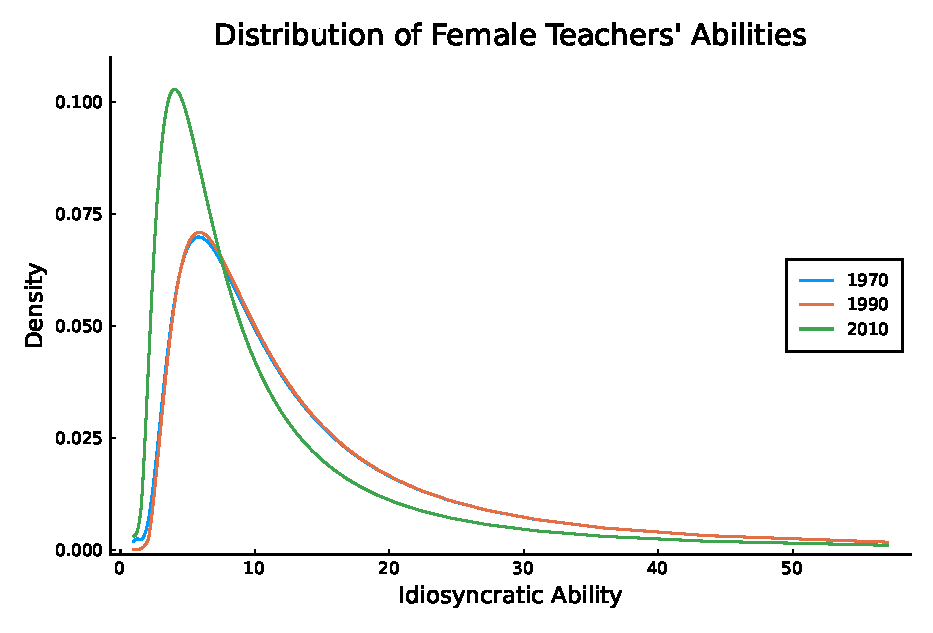
\includegraphics[width=0.8\textwidth]{fT_women_steadystate.eps}
 			\label{ }
 		\end{center}
 	\end{figure}
  \hyperlink{res}{\beamergotobutton{Back}}
\end{frame}

\begin{frame}
\frametitle{Distribution of Teaching Abilities}
\framesubtitle{Male workers with higher abilities become teachers}
\label{maleabil}
\begin{figure}
 		\begin{center}
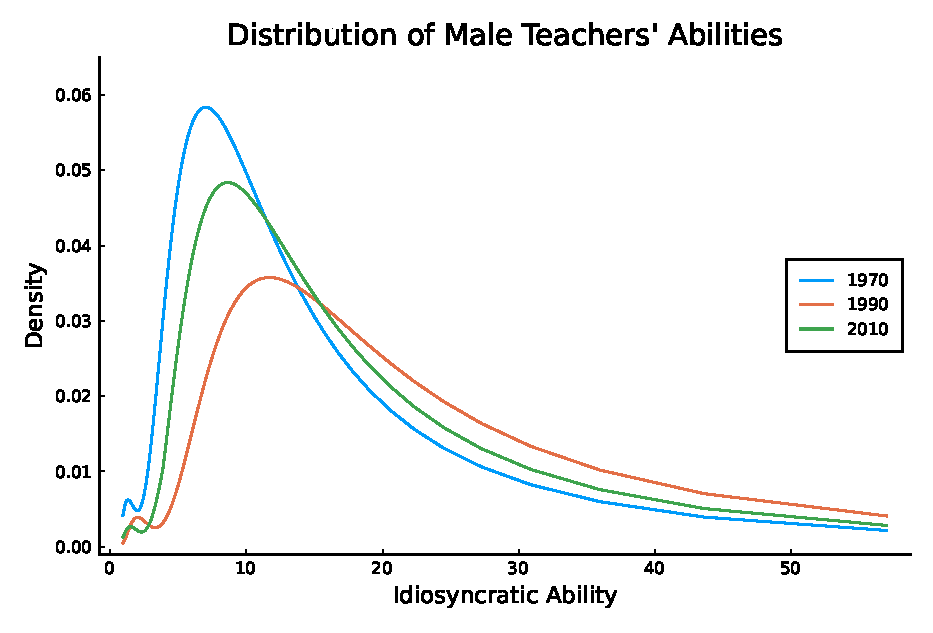
\includegraphics[width=0.8\textwidth]{fT_men_steadystate.eps}
 			\label{ }
 		\end{center}
 	\end{figure}
    \hyperlink{res}{\beamergotobutton{Back}}
\end{frame}

\begin{frame}
\frametitle{Human Capital Investment}
\framesubtitle{Human capital investment decline over time, given ability}
\label{invest}
\begin{figure}
 		\begin{center}
 			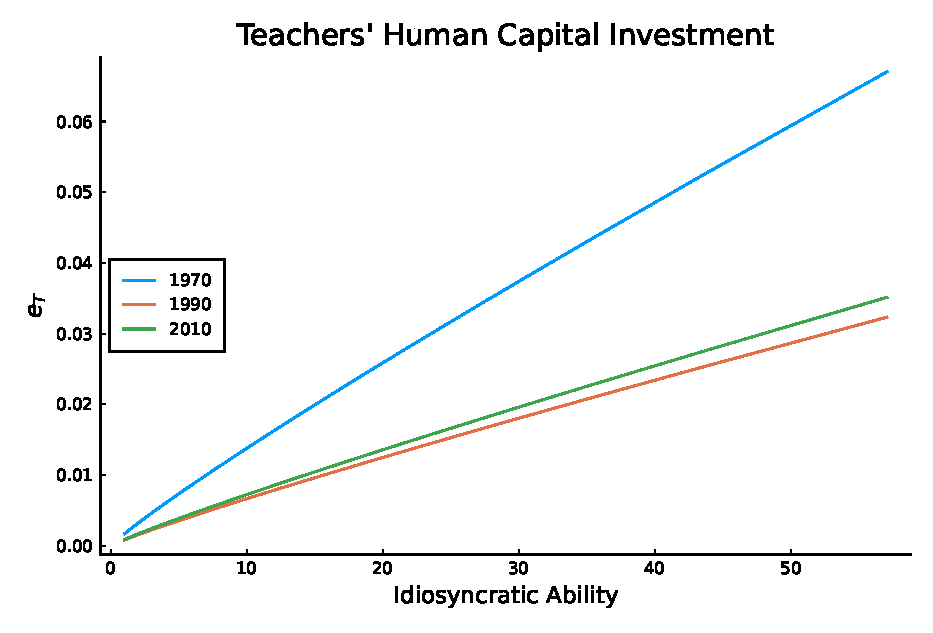
\includegraphics[width=0.8\textwidth]{eT_steadystate.eps}
 			%\caption{ }
 			\label{ }
 		\end{center}
 	\end{figure}
  \hyperlink{res}{\beamergotobutton{Back}}
\end{frame}

\begin{frame}
\frametitle{Human Capital}
\framesubtitle{Values Relative to 1970 Calibration}
\label{humcap}
\begin{table}
  \centering \begin{tabular}{lccc}
\toprule
& 1970 & 1990 & 2010 \\
\midrule
measure of teachers (female) & 1 & 1.000 & 1.765\\
measure of teachers (male) & 1 & 0.462 & 0.731\\
%measure of teachers & 0.031 & 0.023 & 0.040\\
$\widetilde{H}_T^*$ per teacher (female)   & 1 & 0.732 & 0.665 \\
$\widetilde{H}_T^*$ per teacher (male)   & 1 & 1.069 & 1.107 \\
$\widetilde{H}_T^*$ & 1  & 0.620 & 1.002 \\
%$Y_O^*$ & 1 & 0.548 & 0.920 \\
%$\kappa$ & 1.037 & 0.568 & 0.680 \\
\bottomrule
\end{tabular}
%  \caption{ }
\end{table}
 \hyperlink{res}{\beamergotobutton{Back}}
\end{frame}



\begin{frame}
\frametitle{Counterfactual 1: Distribution of Teaching Abilities}
\framesubtitle{Female workers with (relatively) higher abilities become teachers}
\label{counter_femaleabil}
\begin{figure}
 \begin{center}
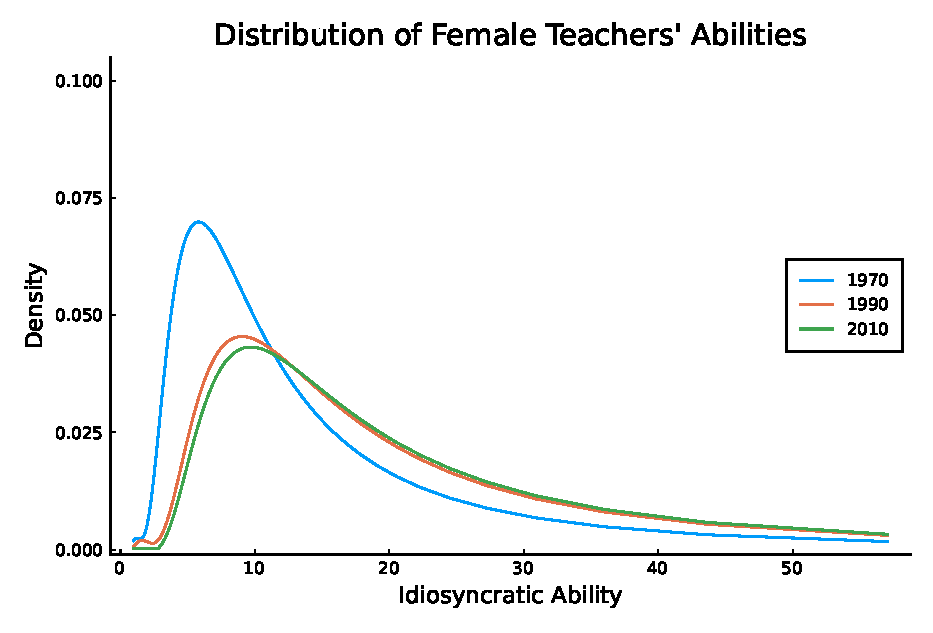
\includegraphics[width=0.8\textwidth]{fT_women_steadystate_counter3.eps}
 			\label{ }
 		\end{center}
 	\end{figure}
   \hyperlink{count}{\beamergotobutton{Back}} \hyperlink{base_femaleabil}{\beamergotobutton{Baseline}}
\end{frame}

\begin{frame}
\frametitle{Counterfactual 1: Distribution of Teaching Abilities}
\framesubtitle{Male workers with (relatively) lower abilities become teachers}
\label{counter_maleabil}
\begin{figure}
 \begin{center}
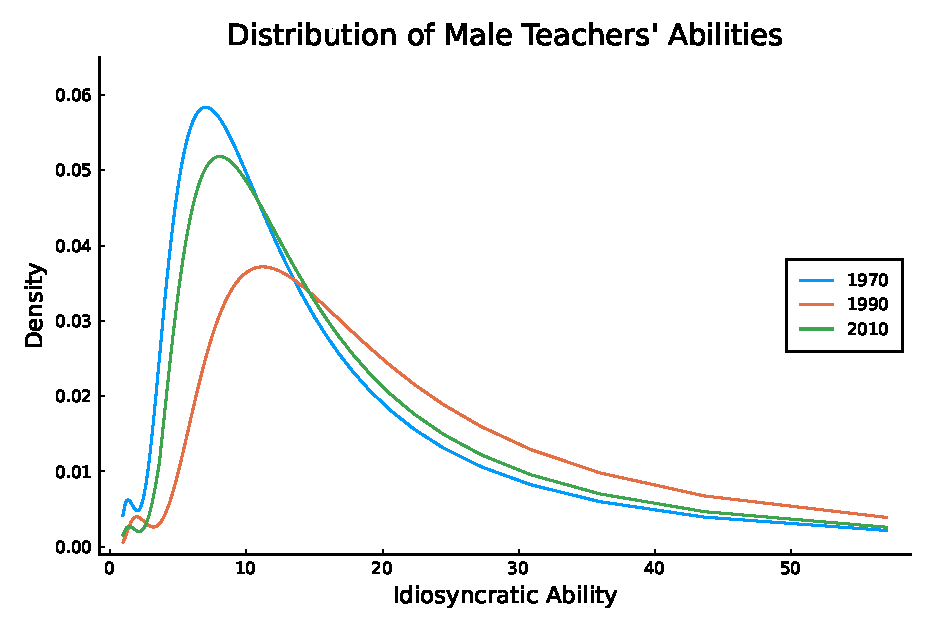
\includegraphics[width=0.8\textwidth]{fT_men_steadystate_counter3.eps}
 			\label{ }
 		\end{center}
 	\end{figure}
   \hyperlink{count}{\beamergotobutton{Back}} \hyperlink{base_maleabil}{\beamergotobutton{Baseline}}
\end{frame}

\begin{frame}
\frametitle{Counterfactual 1: Human Capital Investment}
\framesubtitle{Human capital investment is (relatively) lower, given ability}
\label{counter_invest}
\begin{figure}
 		\begin{center}
 			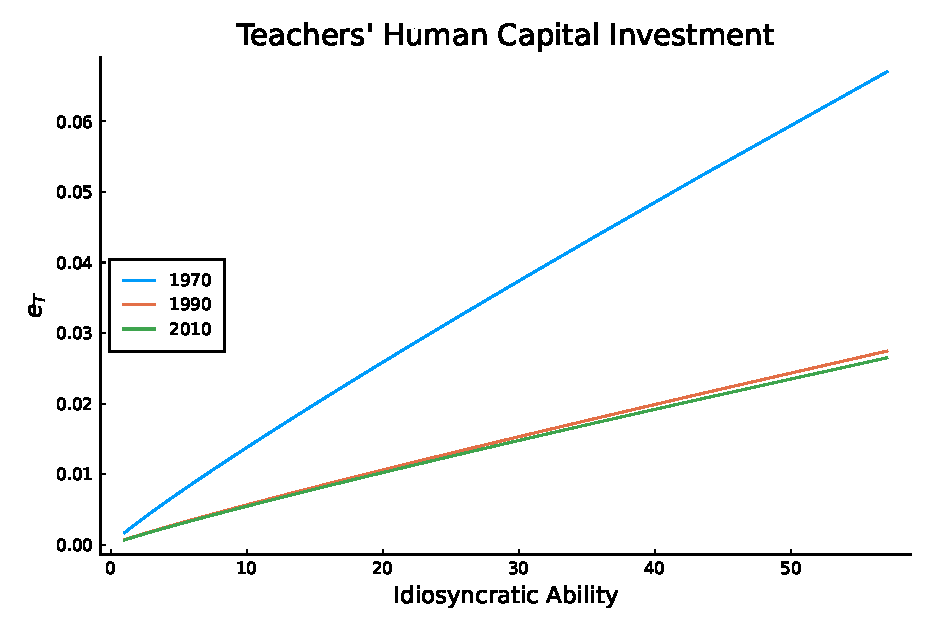
\includegraphics[width=0.8\textwidth]{eT_steadystate_counter3.eps}
 			%\caption{ }
 			\label{ }
 		\end{center}
 	\end{figure}
  \hyperlink{count}{\beamergotobutton{Back}} \hyperlink{base_invest}{\beamergotobutton{Baseline}}
\end{frame}

\begin{frame}
\frametitle{Counterfactual 1: Human Capital}
\framesubtitle{Values Relative to 1970 Benchmark Calibration}
\label{counter_humcap}
\begin{table}
  \centering \begin{tabular}{lccc}
\toprule
& 1970 & 1990 & 2010 \\
\midrule
measure of teachers (female) & 1 & 0.482 & 0.467\\
measure of teachers (male) & 1 & 0.491 & 0.813\\
%measure of teachers & 0.031 & 0.023 & 0.040\\
$\widetilde{H}_T^*$ per teacher (female)   & 1  & 0.908 & 0.991 \\
$\widetilde{H}_T^*$ per teacher (male)   & 1 & 0.851 & 0.739 \\
$\widetilde{H}_T^*$ & 1  & 0.428 & 0.528 \\
%$Y_O^*$ & 1 & 1.058 & 0.638 \\
%$\kappa$ & 1.037 & 0.568 & 0.680 \\
\bottomrule
\end{tabular}
%  \caption{ }
\end{table}
 \hyperlink{count}{\beamergotobutton{Back}}  \hyperlink{base_humcap}{\beamergotobutton{Baseline}}
\end{frame}

% \begin{frame}
% \frametitle{Counterfactual 2: Distribution of Teaching Abilities}
% \framesubtitle{Female workers with (relatively) higher abilities become teachers}
% \label{counter2_femaleabil}
% \begin{figure}
%  \begin{center}
% 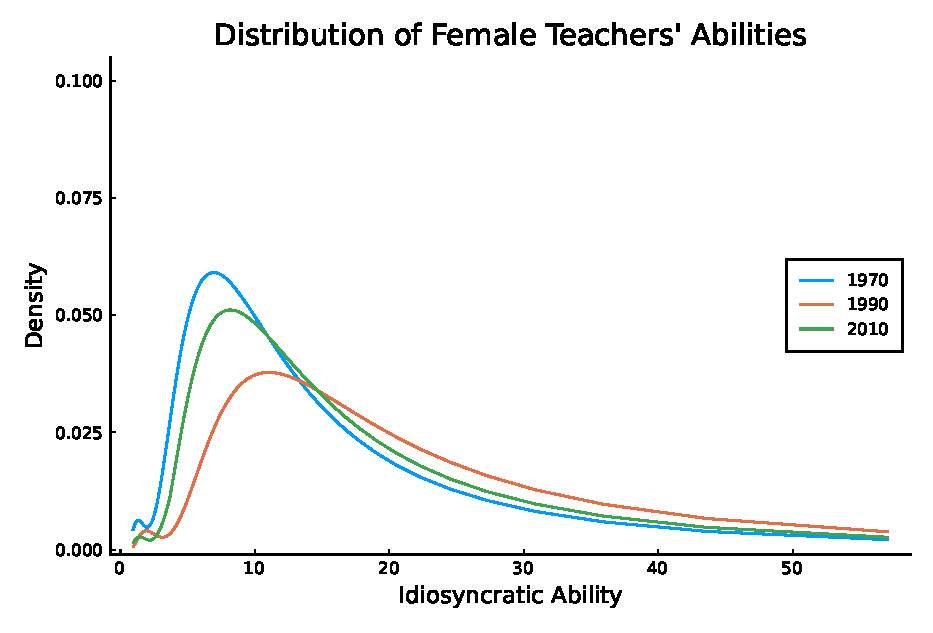
\includegraphics[width=0.8\textwidth]{fT_women_steadystate_counter4.eps}
%  			\label{ }
%  		\end{center}
%  	\end{figure}
%    \hyperlink{count2}{\beamergotobutton{Back}} \hyperlink{base_femaleabil}{\beamergotobutton{Baseline}}
% \end{frame}

% \begin{frame}
% \frametitle{Counterfactual 2: Distribution of Teaching Abilities}
% \framesubtitle{Male workers with (relatively) lower abilities become teachers}
% \label{counter2_maleabil}
% \begin{figure}
%  \begin{center}
% 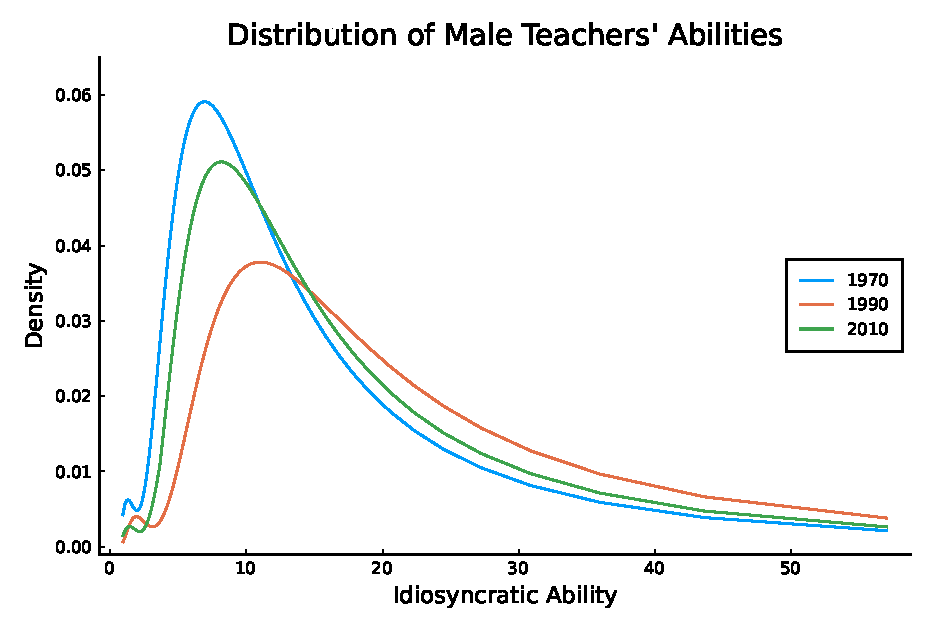
\includegraphics[width=0.8\textwidth]{fT_men_steadystate_counter4.eps}
%  			\label{ }
%  		\end{center}
%  	\end{figure}
%    \hyperlink{count2}{\beamergotobutton{Back}} \hyperlink{base_maleabil}{\beamergotobutton{Baseline}}
% \end{frame}

% \begin{frame}
% \frametitle{Counterfactual 2: Human Capital Investment}
% \framesubtitle{Human capital investment is (relatively) lower, given ability}
% \label{counter2_invest}
% \begin{figure}
%  		\begin{center}
%  			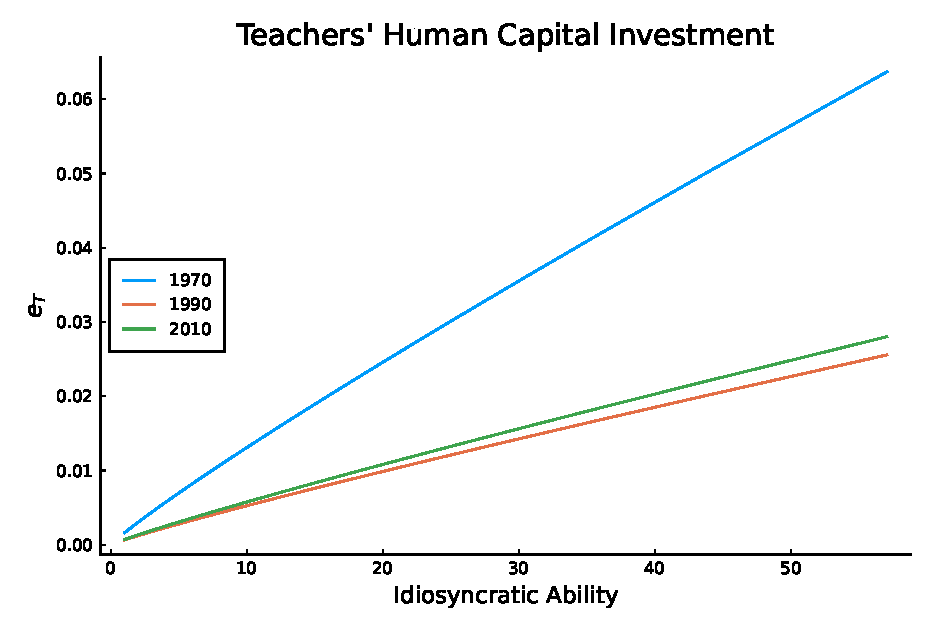
\includegraphics[width=0.8\textwidth]{eT_steadystate_counter4.eps}
%  			%\caption{ }
%  			\label{ }
%  		\end{center}
%  	\end{figure}
%   \hyperlink{count2}{\beamergotobutton{Back}} \hyperlink{base_invest}{\beamergotobutton{Baseline}}
% \end{frame}

% \begin{frame}
% \frametitle{Counterfactual 2: Human Capital}
% \framesubtitle{Values Relative to 1970 Benchmark Calibration}
% \label{counter2_humcap}
% \begin{table}
%   \centering \begin{tabular}{lccc}
% \toprule
% & 1970 & 1990 & 2010 \\
% \midrule
% measure of teachers (female) & 0.781 & 0.385 &0.608\\
% measure of teachers (male) & 1.021 & 0.504 & 0.795\\
% %measure of teachers & 0.031 & 0.023 & 0.040\\
% $\widetilde{H}_T^*$ per teacher (female)    & 1.077 & 0.896 & 0.931 \\
% $\widetilde{H}_T^*$ per teacher (male)    & 0.928 & 0.772 & 0.802 \\
% $\widetilde{H}_T^*$ & 0.891  & 0.366 & 0.600 \\
% %$Y_O^*$ & 1 & 1.058 & 0.638 \\
% %$\kappa$ & 1.037 & 0.568 & 0.680 \\
% \bottomrule
% \end{tabular}
% %  \caption{ }
% \end{table}
%  \hyperlink{count2}{\beamergotobutton{Back}}  \hyperlink{base_humcap}{\beamergotobutton{Baseline}}
% \end{frame}

\begin{frame}
\frametitle{Baseline: Distribution of Teaching Abilities}
\framesubtitle{Female workers with lower abilities become teachers}
\label{base_femaleabil}
\begin{figure}
 \begin{center}
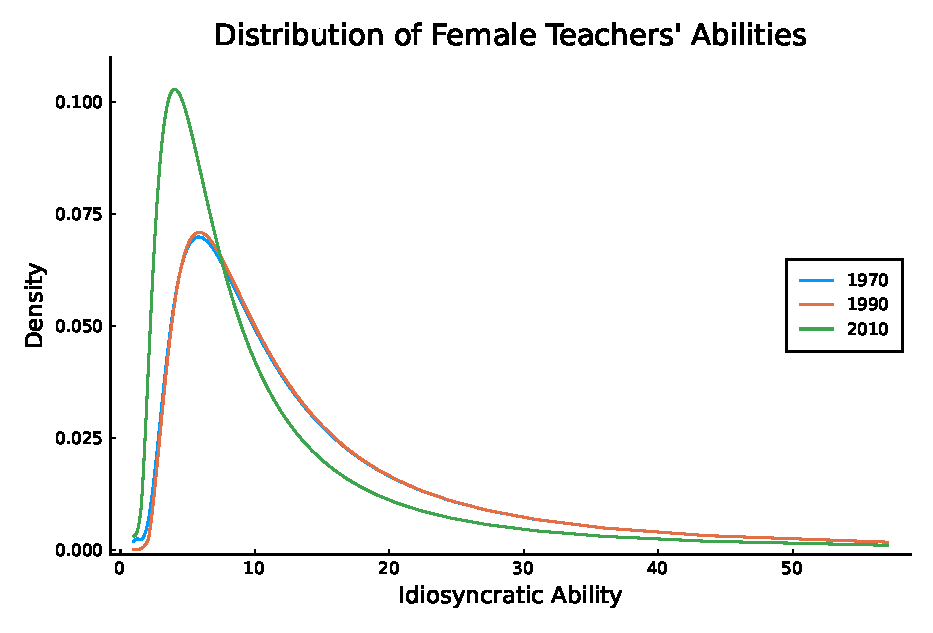
\includegraphics[width=0.8\textwidth]{fT_women_steadystate.eps}
 			\label{ }
 		\end{center}
 	\end{figure}
  \hyperlink{counter_femaleabil}{\beamergotobutton{Counter 1}} %\hyperlink{counter2_femaleabil}{\beamergotobutton{Counter 2}}
\end{frame}

\begin{frame}
\frametitle{Baseline: Distribution of Teaching Abilities}
\framesubtitle{Male workers with higher abilities become teachers}
\label{base_maleabil}
\begin{figure}
 		\begin{center}
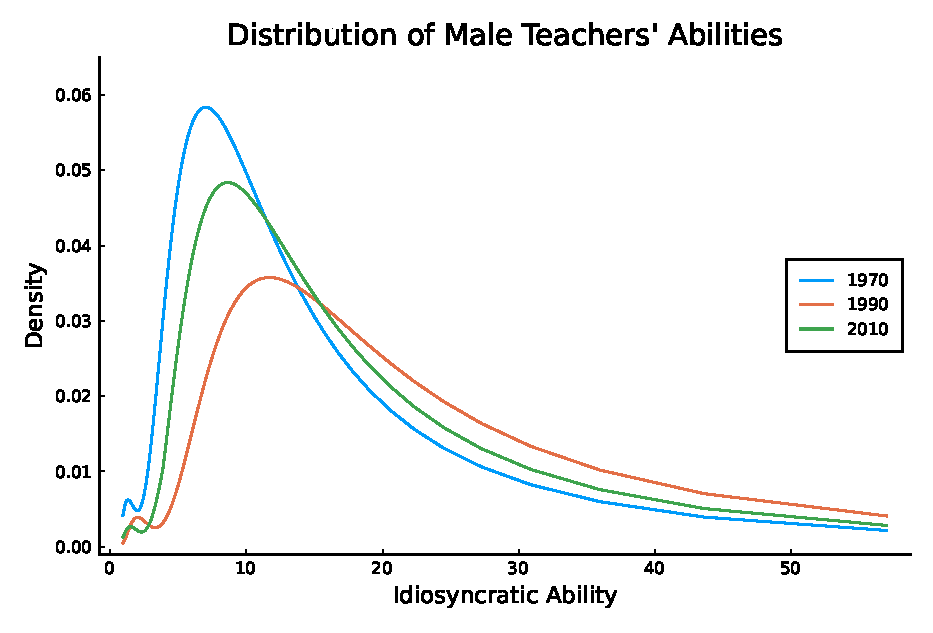
\includegraphics[width=0.8\textwidth]{fT_men_steadystate.eps}
 			\label{ }
 		\end{center}
 	\end{figure}
    \hyperlink{counter_maleabil}{\beamergotobutton{Counter 1}} %\hyperlink{counter2_maleabil}{\beamergotobutton{Counter 2}}
\end{frame}

\begin{frame}
\frametitle{Baseline: Human Capital Investment}
\framesubtitle{Human capital investment decline over time, given ability}
\label{base_invest}
\begin{figure}
 		\begin{center}
 			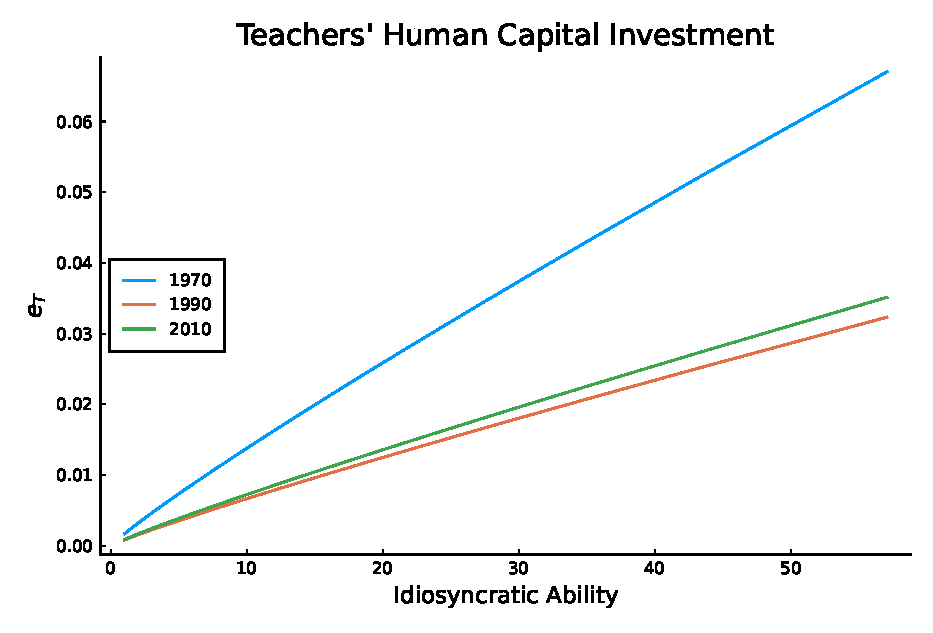
\includegraphics[width=0.8\textwidth]{eT_steadystate.eps}
 			%\caption{ }
 			\label{ }
 		\end{center}
 	\end{figure}
  \hyperlink{counter_invest}{\beamergotobutton{Counter 1}} %\hyperlink{counter2_invest}{\beamergotobutton{Counter 2}}
\end{frame}

\begin{frame}
\frametitle{Baseline: Human Capital}
\framesubtitle{Values Relative to 1970 Calibration}
\label{base_humcap}
\begin{table}
  \centering \begin{tabular}{lccc}
\toprule
& 1970 & 1990 & 2010 \\
\midrule
measure of teachers (female) & 1 & 1.000 & 1.765\\
measure of teachers (male) & 1 & 0.462 & 0.731\\
%measure of teachers & 0.031 & 0.023 & 0.040\\
$\widetilde{H}_T^*$ per teacher (female)   & 1 & 0.732 & 0.665 \\
$\widetilde{H}_T^*$ per teacher (male)   & 1 & 1.069 & 1.107 \\
$\widetilde{H}_T^*$ & 1  & 0.620 & 1.002 \\
%$Y_O^*$ & 1 & 0.548 & 0.920 \\
%$\kappa$ & 1.037 & 0.568 & 0.680 \\
\bottomrule
\end{tabular}
%  \caption{ }
\end{table}
 \hyperlink{counter_humcap}{\beamergotobutton{Counter 1}}  %\hyperlink{counter2_humcap}{\beamergotobutton{Counter 2}}
\end{frame}
\end{document}